\documentclass[11pt]{article}
%Gummi|065|=)
\usepackage{hyperref}
\usepackage{graphicx}
\usepackage{amsmath}
\usepackage{braket}
\usepackage{float}
\begin{document}
\title{Materiales y Diagramas}
\maketitle
\section{Fuente de fotones individuales}

Para realizar el experimento lo primero que se debe preparar, es una fuente de fotones individuales, para realizar esta tarea son necesarios los siguientes materiales

\begin{itemize}
\item Rieles de aluminio
\item Desplazadores milimétricos
\item Postes
\item Filtros infrarrojos 810nm ± 10nm
\item Láser violeta 405nm
\item Láser rojo 700nm
\item Pinholes
\item Cristal BBO-I (Beta Borato de Bario tipo I)
\item Lentes acopladoras
\item Fibras ópticas multimodo
\item 3 Fotodetectores de avalancha
\item Modulo deteccion de fotones individuales multicanal (Single Photon Counting
Module) SPCM
\item Actuador piezoeléctrico 
\item Beam splitter 50:50
\item Beam block
\item irises(no se si se dice asi haga click
\href{https://www.thorlabs.com/thorproduct.cfm?partnumber=ID12 }{aqui})
\end{itemize}

\begin{figure}[H]
\centering
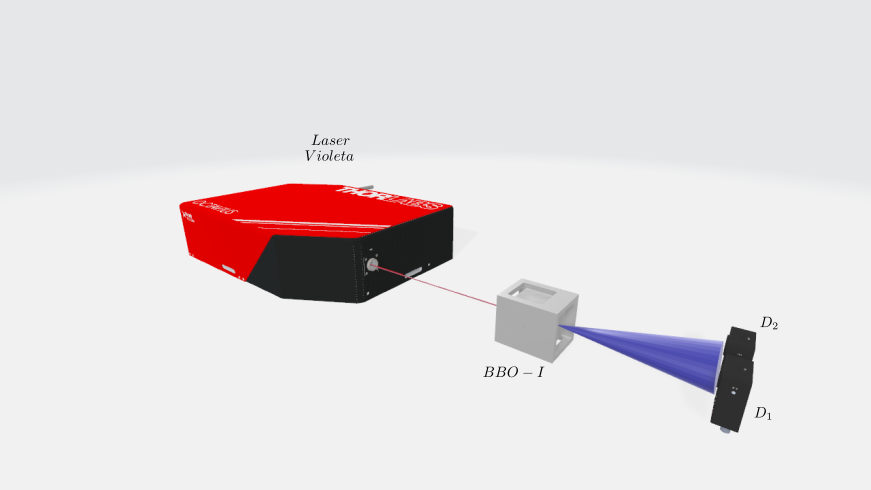
\includegraphics[width=\linewidth]{images/es_acesso.png}
\caption{Arreglo experimental para una fuente de fotones individuales.}
\label{fig:SPDC}
\end{figure}

La figura \ref{fig:SPDC} muestra el arreglo experimental basico para una fuente de fotones individuales, la luz del laser violeta incide sobre el cristal BBO-I produciendo dos fotones individuales que viajan por distintos caminos, uno de ellos se utiliza como testigo para verificar que se tienen fotones individuales, se indica que se produjo un par de fotones cuando ambos detectores hacen click en una ventana temporal a determinar
 
En este montaje se mide, lo que conoce como funcion de correlacion de glauber $\alpha_{2d}$ \cite{pearson} que esta dado por:

\begin{equation}
\alpha_{2d}=\frac{R_{c}}{\tau_{c}R_{1} R_{2}}
\end{equation}

Donde $R_{1}$ es el promedio  de conteos en el detector 1, $R_{2}$ en el detector 2, $R_{c}$ es el promedio de conteos que coindicen temporalmente entre $D_{1}$ y $D_{2}$  y $\tau_{c}$ es la ventana temporal en la cual las detecciones se concideran como coincidencias

Para eliminar coincidencias accidentales del montaje anterior, se mide la funcion de correlaccion de glauber a tres detectores mediante el siguiente arreglo experimental


\begin{figure}[H]
\centering
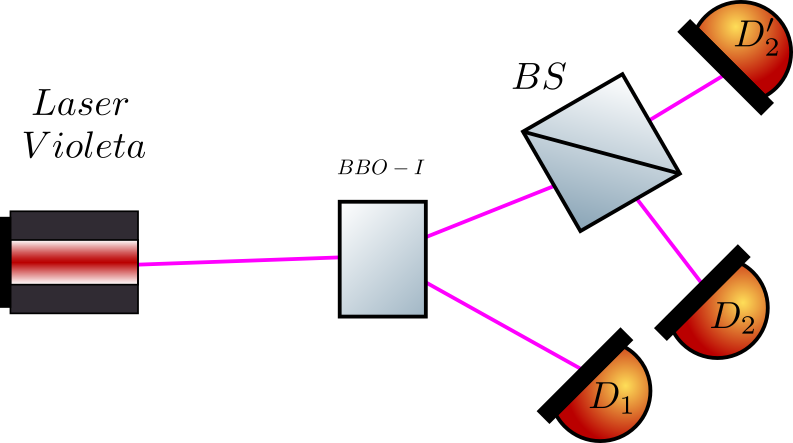
\includegraphics[width=\linewidth]{images/acceso.png}
\caption{Arreglo experimental para eliminar las coincidencias accidentales en una fuente de fotones individuales.}
\label{fig:SPDC2}
\end{figure}

\begin{equation}
\alpha_{3d}=\frac{R_{122'}}{R_{12}R_{12'}}R_{1}
\end{equation}


\section{Interferometro de Mach-Zehnder y mediciones sin interaccion}


El siguiente paso es montar un interferometro de Mach-Zehnder, para ello en adicion a los materiales de la seccion anterior son necesarios los siguientes

\begin{itemize}
\item Beam splitters de distintos valores tantos como sea posible
\item Polarizadores
\item Retardadores de fase
\item Chopper optico
\item Espejos
\item Fuente de luz incandescente
\end{itemize}

El arreglo experimental a realizar es el siguiente


\begin{figure}[H]
\centering
\includegraphics[scale=0.5]{images/machzehnder_single.png}
\caption{Arreglo experimental De un interferometro de Mach-Zehnder.}
\label{fig:SPDC3}
\end{figure}

Las mediciones sin interaccion consisten en este mismo arreglo experimental con un objeto en uno de los brazos del interferometro como lo muestra la siguiente figura


\begin{figure}[H]
\centering
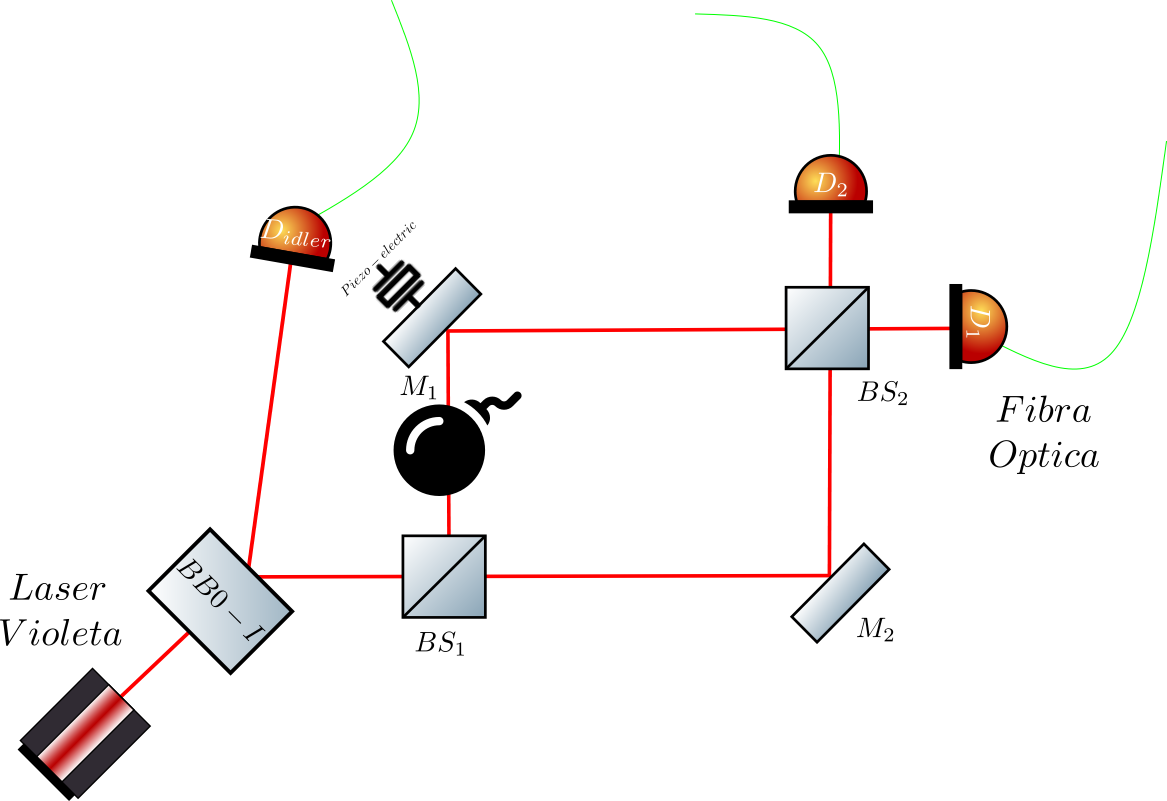
\includegraphics[scale=0.5]{images/machzehnder_single_es_b.png}
\caption{Arreglo experimental mediciones sin interaccion.}
\label{fig:SPDC5}
\end{figure}

Como obstaculo, el cual es ilustrado por una bomba se usaran los polarizadores y los retardadores de fase, la ley de malus nos da una manera de controlar la transparencia de los polarizadores, de igual manera los retardadores de fase nos permiten cambiar la fase que induce el objeto.

Luego de haber realizado las mediciones con estos objetos se usa un chopper optico como obstaculo


\bibliography{bibliography.bib}
\bibliographystyle{unsrt}




\end{document}
